\documentclass{article}

\usepackage[utf8]{inputenc}
\usepackage{tikz}

\setlength{\parindent}{0pt}

\tikzset{state/.style={draw,circle}}

\usetikzlibrary{arrows, automata}
\usetikzlibrary{positioning}

%**************************************************
% Node definitions for figures
%**************************************************
% Black node 
\tikzstyle{black_node} = [
    circle, 
    white, 
    font=\bfseries, 
    draw=black, 
    fill=black, 
    align=center, 
    inner sep=2pt, % 2pt is good for two digits
    text width=1.5em, 
    text centered
]

% Red node
\tikzstyle{red_node} = [
    circle, 
    white, 
    font=\bfseries, 
    draw=black,
    fill=red,
    align=center, 
    inner sep=2pt, % 2pt is good for two digits
    text width=1.5em, 
    text centered
]

% NIL node - drawn as black rounded rectangles
\tikzstyle{nil} = [
    rounded corners, 
    white,
    draw=black, 
    fill=black,
    align=center, 
    inner sep=0pt, 
    minimum width=1.0em, 
    minimum height=1.0em
]

\begin{document}

\textbf{CLRS Problem 13.4-3:} delete nodes from the red-black tree created in problem 13.3-2.
\\ \\
%**************************************************
% Problem 13.4-3
%**************************************************
\textbf{\emph{Note: NIL nodes shown as black rounded-corner rectangles.}}
\\ \\
%--------------------------------------------------
% 8
%--------------------------------------------------
\textbf{Delete: 8}
\\ 
Start with the red-black tree from the insert exercise.
\\ \\
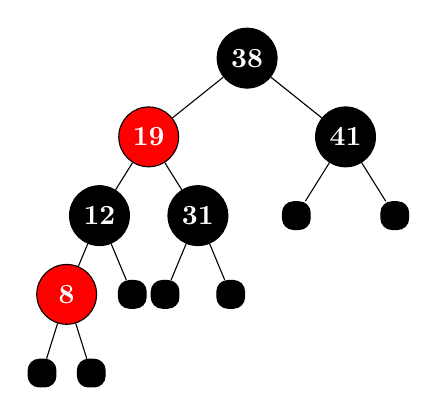
\begin{tikzpicture}[
    level/.style={
        sibling distance = 2.5cm/#1, 
        level distance = 1.00cm
    }
] 
\node [black_node] {38}
    child{ node [red_node] {19}
        child{ node [black_node] {12}
            child{ node [red_node] {8}
                child{ node [nil] {}}
                child{ node [nil] {}}
            }
            child{ node [nil] {}}
        }
        child{ node [black_node] {31}
            child{ node [nil] {}}
            child{ node [nil] {}}
        }
    }
    child{ node [black_node] {41}
        child{ node [nil] {}}
        child{ node [nil] {}}
    }
; 
\end{tikzpicture}
\\ \\
Now, deleting a red node is easy, just remove it, replace it with a nil node.
\\ \\
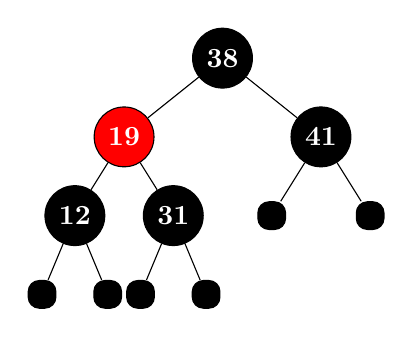
\begin{tikzpicture}[
    level/.style={
        sibling distance = 2.5cm/#1, 
        level distance = 1.00cm
    }
] 
\node [black_node] {38}
    child{ node [red_node] {19}
        child{ node [black_node] {12}
            child{ node [nil] {}}
            child{ node [nil] {}}
        }
        child{ node [black_node] {31}
            child{ node [nil] {}}
            child{ node [nil] {}}
        }
    }
    child{ node [black_node] {41}
        child{ node [nil] {}}
        child{ node [nil] {}}
    }
; 
\end{tikzpicture}
\\ \\ \\
%--------------------------------------------------
% 12
%--------------------------------------------------
\textbf{Delete: 12}
\\
Recolor parent and silbing of deleted node (now a nil node).
\\ \\
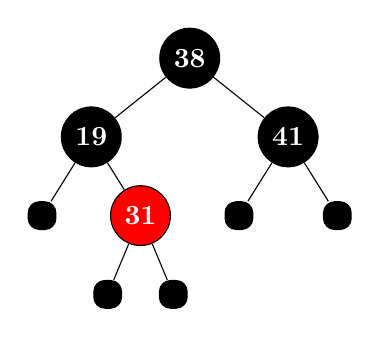
\begin{tikzpicture}[
    level/.style={
        sibling distance = 2.5cm/#1, 
        level distance = 1.00cm
    }
] 
\node [black_node] {38}
    child{ node [black_node] {19}
        child{ node [nil] {}}
        child{ node [red_node] {31}
            child{ node [nil] {}}
            child{ node [nil] {}}
        }
    }
    child{ node [black_node] {41}
        child{ node [nil] {}}
        child{ node [nil] {}}
    }
; 
\end{tikzpicture}
\\ \\ \\
%--------------------------------------------------
% 19
%--------------------------------------------------
\textbf{Delete: 19}
\\
Connect single child to grandparent, and recolor this node to preserve the black height.
\\ \\
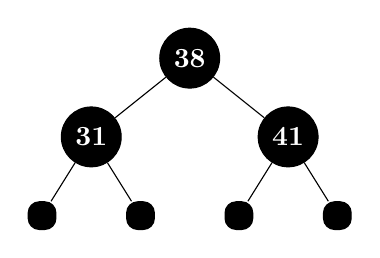
\begin{tikzpicture}[
    level/.style={
        sibling distance = 2.5cm/#1, 
        level distance = 1.00cm
    }
] 
\node [black_node] {38}
    child{ node [black_node] {31}
        child{ node [nil] {}}
        child{ node [nil] {}}
    }
    child{ node [black_node] {41}
        child{ node [nil] {}}
        child{ node [nil] {}}
    }
; 
\end{tikzpicture}
\\ \\ \\
%--------------------------------------------------
% 31
%--------------------------------------------------
\textbf{Delete: 31}
\\
Deleting node with key 31 gives
\\ \\
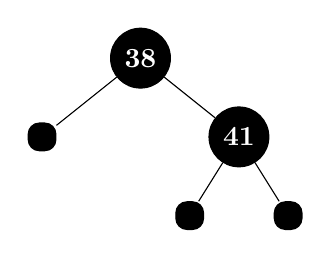
\begin{tikzpicture}[
    level/.style={
        sibling distance = 2.5cm/#1, 
        level distance = 1.00cm
    }
] 
\node [black_node] {38}
    child{ node [nil] {}}
    child{ node [black_node] {41}
        child{ node [nil] {}}
        child{ node [nil] {}}
    }
; 
\end{tikzpicture}
\\ \\
Now, recolor sibling to restore black height.
\\ \\
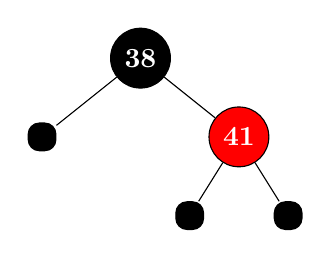
\begin{tikzpicture}[
    level/.style={
        sibling distance = 2.5cm/#1, 
        level distance = 1.00cm
    }
] 
\node [black_node] {38}
    child{ node [nil] {}}
    child{ node [red_node] {41}
        child{ node [nil] {}}
        child{ node [nil] {}}
    }
; 
\end{tikzpicture}

\newpage

%--------------------------------------------------
% 38
%--------------------------------------------------
\textbf{Delete: 38}
\\
Deleting the root with key 38 gives
\\ \\
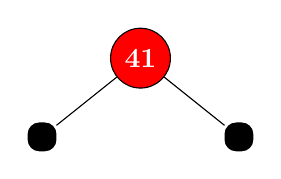
\begin{tikzpicture}[
    level/.style={
        sibling distance = 2.5cm/#1, 
        level distance = 1.00cm
    }
] 
\node [red_node] {41}
    child{ node [nil] {}}
    child{ node [nil] {}}
; 
\end{tikzpicture}
\\ \\
Of course, the root must be black, recolor the root.
\\ \\
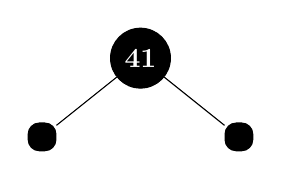
\begin{tikzpicture}[
    level/.style={
        sibling distance = 2.5cm/#1, 
        level distance = 1.00cm
    }
] 
\node [black_node] {41}
    child{ node [nil] {}}
    child{ node [nil] {}}
; 
\end{tikzpicture}
\\ \\ \\
%--------------------------------------------------
% 41
%--------------------------------------------------
\textbf{Delete: 41}
\\
Deleting the root gives an empty tree.
\\ \\
Done!

\end{document}